\documentclass[]{article}
\usepackage{lmodern}
\usepackage{amssymb,amsmath}
\usepackage{ifxetex,ifluatex}
\usepackage{fixltx2e} % provides \textsubscript
\ifnum 0\ifxetex 1\fi\ifluatex 1\fi=0 % if pdftex
  \usepackage[T1]{fontenc}
  \usepackage[utf8]{inputenc}
\else % if luatex or xelatex
  \ifxetex
    \usepackage{mathspec}
  \else
    \usepackage{fontspec}
  \fi
  \defaultfontfeatures{Ligatures=TeX,Scale=MatchLowercase}
\fi
% use upquote if available, for straight quotes in verbatim environments
\IfFileExists{upquote.sty}{\usepackage{upquote}}{}
% use microtype if available
\IfFileExists{microtype.sty}{%
\usepackage{microtype}
\UseMicrotypeSet[protrusion]{basicmath} % disable protrusion for tt fonts
}{}
\usepackage[margin=1in]{geometry}
\usepackage{hyperref}
\hypersetup{unicode=true,
            pdftitle={Data Visualization in R},
            pdfauthor={Umair Durrani},
            pdfborder={0 0 0},
            breaklinks=true}
\urlstyle{same}  % don't use monospace font for urls
\usepackage{graphicx,grffile}
\makeatletter
\def\maxwidth{\ifdim\Gin@nat@width>\linewidth\linewidth\else\Gin@nat@width\fi}
\def\maxheight{\ifdim\Gin@nat@height>\textheight\textheight\else\Gin@nat@height\fi}
\makeatother
% Scale images if necessary, so that they will not overflow the page
% margins by default, and it is still possible to overwrite the defaults
% using explicit options in \includegraphics[width, height, ...]{}
\setkeys{Gin}{width=\maxwidth,height=\maxheight,keepaspectratio}
\IfFileExists{parskip.sty}{%
\usepackage{parskip}
}{% else
\setlength{\parindent}{0pt}
\setlength{\parskip}{6pt plus 2pt minus 1pt}
}
\setlength{\emergencystretch}{3em}  % prevent overfull lines
\providecommand{\tightlist}{%
  \setlength{\itemsep}{0pt}\setlength{\parskip}{0pt}}
\setcounter{secnumdepth}{0}
% Redefines (sub)paragraphs to behave more like sections
\ifx\paragraph\undefined\else
\let\oldparagraph\paragraph
\renewcommand{\paragraph}[1]{\oldparagraph{#1}\mbox{}}
\fi
\ifx\subparagraph\undefined\else
\let\oldsubparagraph\subparagraph
\renewcommand{\subparagraph}[1]{\oldsubparagraph{#1}\mbox{}}
\fi

%%% Use protect on footnotes to avoid problems with footnotes in titles
\let\rmarkdownfootnote\footnote%
\def\footnote{\protect\rmarkdownfootnote}

%%% Change title format to be more compact
\usepackage{titling}

% Create subtitle command for use in maketitle
\providecommand{\subtitle}[1]{
  \posttitle{
    \begin{center}\large#1\end{center}
    }
}

\setlength{\droptitle}{-2em}

  \title{Data Visualization in R}
    \pretitle{\vspace{\droptitle}\centering\huge}
  \posttitle{\par}
    \author{Umair Durrani}
    \preauthor{\centering\large\emph}
  \postauthor{\par}
      \predate{\centering\large\emph}
  \postdate{\par}
    \date{2019-06-24}

\usepackage{booktabs}
\usepackage{longtable}
\usepackage{array}
\usepackage{multirow}
\usepackage{wrapfig}
\usepackage{float}
\usepackage{colortbl}
\usepackage{pdflscape}
\usepackage{tabu}
\usepackage{threeparttable}
\usepackage{threeparttablex}
\usepackage[normalem]{ulem}
\usepackage{makecell}
\usepackage{xcolor}

\begin{document}
\maketitle

{
\setcounter{tocdepth}{2}
\tableofcontents
}
\hypertarget{load-libraries}{%
\section{Load libraries}\label{load-libraries}}


\includegraphics{/cloud/project/figures/data.png}

\hypertarget{load-data}{%
\section{Load data}\label{load-data}}

\begin{quote}
An excerpt of the data available at Gapminder.org. For each of 142
countries, the package provides values for life expectancy, GDP per
capita, and population, every five years, from 1952 to 2007.
\end{quote}

\hypertarget{exploratory-data-analysis}{%
\section{Exploratory Data Analysis}\label{exploratory-data-analysis}}

\hypertarget{data-structure}{%
\subsection{Data structure}\label{data-structure}}

\begin{verbatim}
## Observations: 1,704
## Variables: 6
## $ country   <fct> Afghanistan, Afghanistan, Afghanistan, Afghanistan, ...
## $ continent <fct> Asia, Asia, Asia, Asia, Asia, Asia, Asia, Asia, Asia...
## $ year      <int> 1952, 1957, 1962, 1967, 1972, 1977, 1982, 1987, 1992...
## $ lifeExp   <dbl> 28.801, 30.332, 31.997, 34.020, 36.088, 38.438, 39.8...
## $ pop       <int> 8425333, 9240934, 10267083, 11537966, 13079460, 1488...
## $ gdpPercap <dbl> 779.4453, 820.8530, 853.1007, 836.1971, 739.9811, 78...
\end{verbatim}

\textbf{First 10 rows}

\begin{table}[H]
\centering
\begin{tabular}{l|l|r|r|r|r}
\hline
country & continent & year & lifeExp & pop & gdpPercap\\
\hline
Afghanistan & Asia & 1952 & 28.801 & 8425333 & 779.4453\\
\hline
Afghanistan & Asia & 1957 & 30.332 & 9240934 & 820.8530\\
\hline
Afghanistan & Asia & 1962 & 31.997 & 10267083 & 853.1007\\
\hline
Afghanistan & Asia & 1967 & 34.020 & 11537966 & 836.1971\\
\hline
Afghanistan & Asia & 1972 & 36.088 & 13079460 & 739.9811\\
\hline
Afghanistan & Asia & 1977 & 38.438 & 14880372 & 786.1134\\
\hline
Afghanistan & Asia & 1982 & 39.854 & 12881816 & 978.0114\\
\hline
Afghanistan & Asia & 1987 & 40.822 & 13867957 & 852.3959\\
\hline
Afghanistan & Asia & 1992 & 41.674 & 16317921 & 649.3414\\
\hline
Afghanistan & Asia & 1997 & 41.763 & 22227415 & 635.3414\\
\hline
\end{tabular}
\end{table}

\begin{verbatim}
## Skim summary statistics
##  n obs: 1704 
##  n variables: 6 
## 
## -- Variable type:factor --------------------------------------------------------------------------------------------------
##   variable missing complete    n n_unique
##  continent       0     1704 1704        5
##    country       0     1704 1704      142
##                              top_counts ordered
##  Afr: 624, Asi: 396, Eur: 360, Ame: 300   FALSE
##      Afg: 12, Alb: 12, Alg: 12, Ang: 12   FALSE
## 
## -- Variable type:integer -------------------------------------------------------------------------------------------------
##  variable missing complete    n    mean       sd    p0        p25     p50
##       pop       0     1704 1704 3e+07    1.1e+08 60011 2793664    7e+06  
##      year       0     1704 1704  1979.5 17.27     1952    1965.75  1979.5
##       p75       p100     hist
##  2e+07       1.3e+09 ▇▁▁▁▁▁▁▁
##   1993.25 2007       ▇▃▇▃▃▇▃▇
## 
## -- Variable type:numeric -------------------------------------------------------------------------------------------------
##   variable missing complete    n    mean      sd     p0     p25     p50
##  gdpPercap       0     1704 1704 7215.33 9857.45 241.17 1202.06 3531.85
##    lifeExp       0     1704 1704   59.47   12.92  23.6    48.2    60.71
##      p75      p100     hist
##  9325.46 113523.13 ▇▁▁▁▁▁▁▁
##    70.85     82.6  ▁▂▅▅▅▅▇▃
\end{verbatim}

\hypertarget{using-ggplot2-library-for-plotting}{%
\section{Using ggplot2 library for
plotting}\label{using-ggplot2-library-for-plotting}}

\begin{quote}
ggplot2 is the name of a library in R language that is used for
plotting. It is a part of the \texttt{tidyverse} library that contains
other libraries for \emph{tidy} data analysis.
\end{quote}

When we ran \texttt{library(tidyverse)}, the \texttt{ggplot2} library
was also loaded. If we only want to load \texttt{ggplot2}, we can do so:

\hypertarget{filtering-the-gapminder-data-for-canada}{%
\subsection{\texorpdfstring{Filtering the \texttt{gapminder} data for
\textbf{Canada}}{Filtering the gapminder data for Canada}}\label{filtering-the-gapminder-data-for-canada}}

\textbf{Pseudo code} 1. Take the gapminder data \emph{AND THEN} 2.
Filter out all the data except for Canada

\textbf{R code}

\begin{verbatim}
## # A tibble: 12 x 6
##    country continent  year lifeExp      pop gdpPercap
##    <fct>   <fct>     <int>   <dbl>    <int>     <dbl>
##  1 Canada  Americas   1952    68.8 14785584    11367.
##  2 Canada  Americas   1957    70.0 17010154    12490.
##  3 Canada  Americas   1962    71.3 18985849    13462.
##  4 Canada  Americas   1967    72.1 20819767    16077.
##  5 Canada  Americas   1972    72.9 22284500    18971.
##  6 Canada  Americas   1977    74.2 23796400    22091.
##  7 Canada  Americas   1982    75.8 25201900    22899.
##  8 Canada  Americas   1987    76.9 26549700    26627.
##  9 Canada  Americas   1992    78.0 28523502    26343.
## 10 Canada  Americas   1997    78.6 30305843    28955.
## 11 Canada  Americas   2002    79.8 31902268    33329.
## 12 Canada  Americas   2007    80.7 33390141    36319.
\end{verbatim}


\includegraphics{/cloud/project/figures/layered_graphics.png}

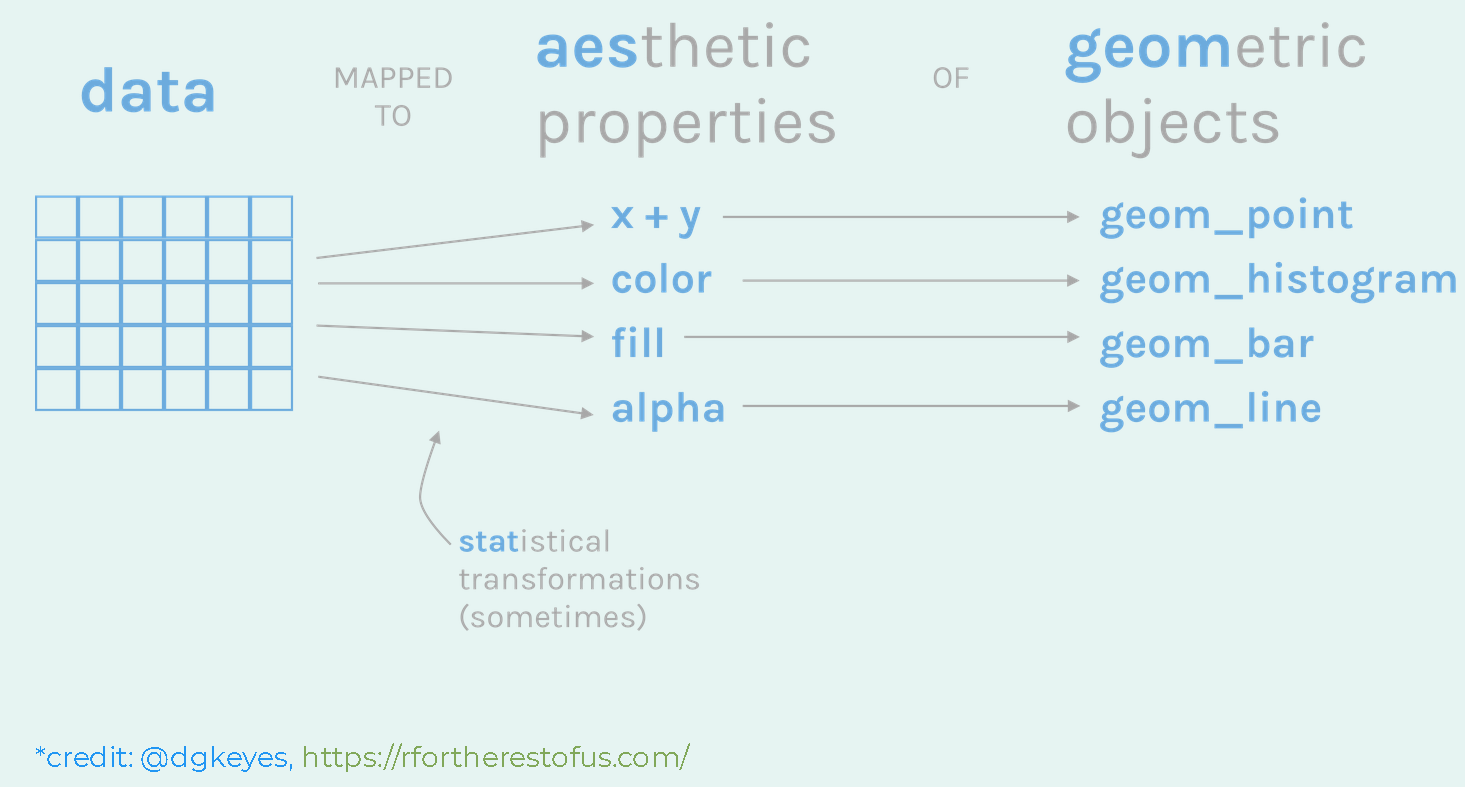
\includegraphics{/cloud/project/figures/layered.PNG}

\hypertarget{plotting-population-over-years}{%
\subsection{Plotting population over
years}\label{plotting-population-over-years}}

\textbf{data}
\includegraphics{Using_ggplot2_files/figure-latex/unnamed-chunk-9-1.pdf}

\textbf{data and aesthetics}
\includegraphics{Using_ggplot2_files/figure-latex/unnamed-chunk-10-1.pdf}

\textbf{data, aesthetics and geometric object}
\includegraphics{Using_ggplot2_files/figure-latex/unnamed-chunk-11-1.pdf}

\begin{quote}
YOUR TURN: Create a new data set for your favorite country and plot its
population over years
\end{quote}


\includegraphics{/cloud/project/figures/more_aesthetics.png}

\hypertarget{color}{%
\subsection{Color}\label{color}}

\hypertarget{numeric}{%
\subsubsection{Numeric}\label{numeric}}

\includegraphics{Using_ggplot2_files/figure-latex/unnamed-chunk-13-1.pdf}

\hypertarget{categories}{%
\subsubsection{Categories}\label{categories}}

\includegraphics{Using_ggplot2_files/figure-latex/unnamed-chunk-14-1.pdf}

\hypertarget{size}{%
\subsection{Size}\label{size}}

\includegraphics{Using_ggplot2_files/figure-latex/unnamed-chunk-15-1.pdf}

\hypertarget{shape-not-great-for-3-categories}{%
\subsection{Shape (Not great for \textgreater{} 3
categories)}\label{shape-not-great-for-3-categories}}

\begin{verbatim}
## Warning: The shape palette can deal with a maximum of 6 discrete values
## because more than 6 becomes difficult to discriminate; you have
## 12. Consider specifying shapes manually if you must have them.
\end{verbatim}

\begin{verbatim}
## Warning: Removed 6 rows containing missing values (geom_point).
\end{verbatim}

\includegraphics{Using_ggplot2_files/figure-latex/unnamed-chunk-16-1.pdf}

\hypertarget{what-if-you-use-all}{%
\subsection{What if you use all?}\label{what-if-you-use-all}}

\includegraphics{Using_ggplot2_files/figure-latex/unnamed-chunk-17-1.pdf}

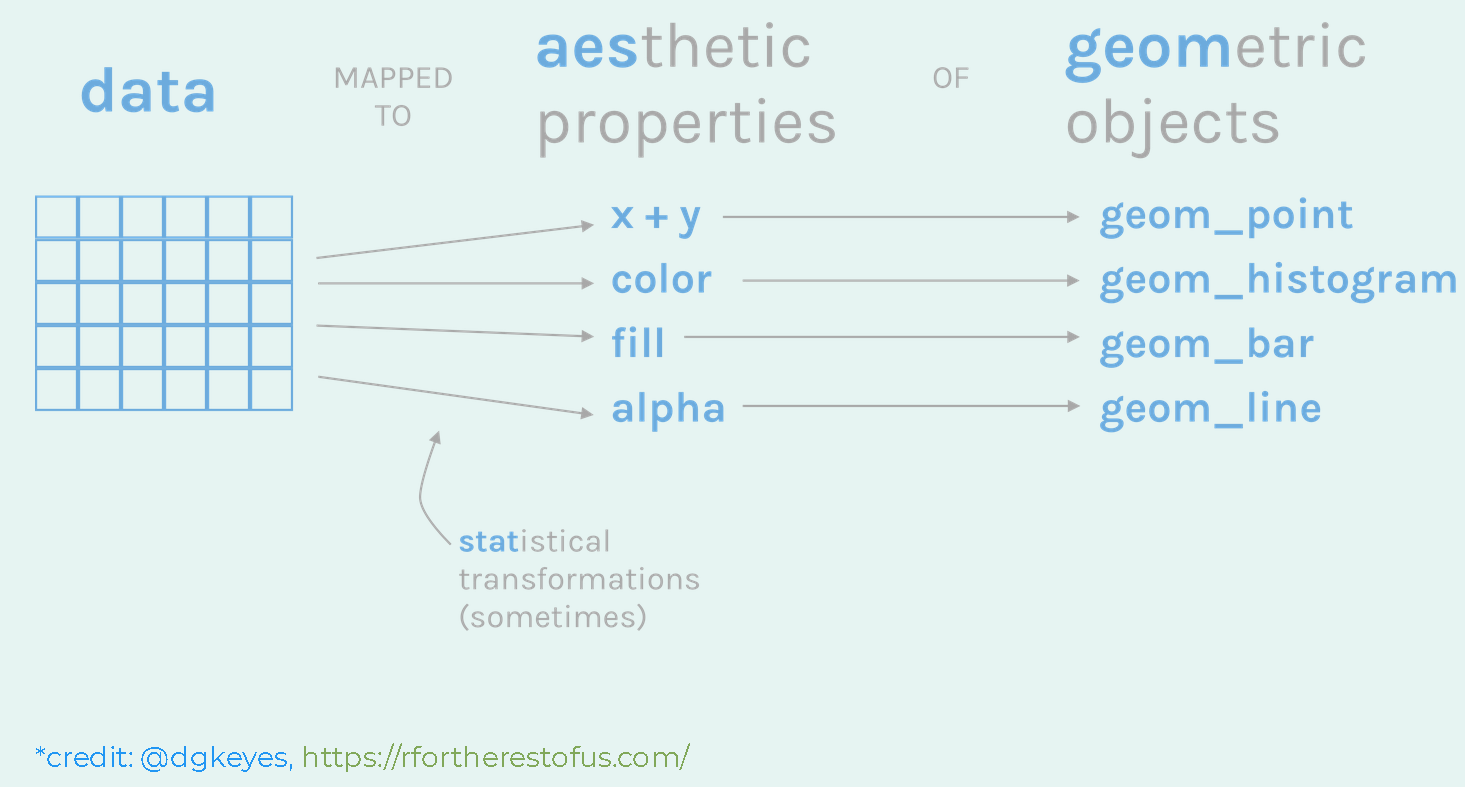
\includegraphics{/cloud/project/figures/layered.PNG}


\includegraphics{/cloud/project/figures/geoms.png}

\hypertarget{line}{%
\subsection{Line}\label{line}}

\includegraphics{Using_ggplot2_files/figure-latex/unnamed-chunk-18-1.pdf}

\hypertarget{histogram}{%
\subsection{Histogram}\label{histogram}}

Now using the compete \texttt{gapminder} data:

\begin{verbatim}
## `stat_bin()` using `bins = 30`. Pick better value with `binwidth`.
\end{verbatim}

\includegraphics{Using_ggplot2_files/figure-latex/unnamed-chunk-19-1.pdf}

\hypertarget{fill-color}{%
\subsubsection{fill color}\label{fill-color}}

\begin{verbatim}
## `stat_bin()` using `bins = 30`. Pick better value with `binwidth`.
\end{verbatim}

\includegraphics{Using_ggplot2_files/figure-latex/unnamed-chunk-20-1.pdf}

\textbf{add transparency}

\begin{verbatim}
## `stat_bin()` using `bins = 30`. Pick better value with `binwidth`.
\end{verbatim}

\includegraphics{Using_ggplot2_files/figure-latex/unnamed-chunk-21-1.pdf}

\hypertarget{boxplot}{%
\subsection{Boxplot}\label{boxplot}}

\includegraphics{Using_ggplot2_files/figure-latex/unnamed-chunk-22-1.pdf}

\hypertarget{creating-a-scatter-plot-for-all-countries}{%
\subsection{Creating a scatter plot for all
countries}\label{creating-a-scatter-plot-for-all-countries}}

Now we'll use the complete \texttt{gapminder} data
\includegraphics{Using_ggplot2_files/figure-latex/unnamed-chunk-23-1.pdf}

\begin{quote}
YOUR TURN: Copy the above code and paste it below. Replace \texttt{year}
with \texttt{gdpPercap}
\end{quote}

\textbf{Colour the continents}
\includegraphics{Using_ggplot2_files/figure-latex/unnamed-chunk-25-1.pdf}

\begin{quote}
YOUR TURN: Copy the above code and paste in the R chunk below. Then
change \texttt{color}to \texttt{size} and run it.
\end{quote}


\includegraphics{/cloud/project/figures/facets.png}

\textbf{Separate the continents using \texttt{facets}}
\includegraphics{Using_ggplot2_files/figure-latex/unnamed-chunk-27-1.pdf}

\textbf{Change scales}
\includegraphics{Using_ggplot2_files/figure-latex/unnamed-chunk-28-1.pdf}

\textbf{Can we create a facet for each country?} \textgreater{} YES

\includegraphics{Using_ggplot2_files/figure-latex/unnamed-chunk-29-1.pdf}

\includegraphics{https://media.giphy.com/media/gS2l5jPcE0F4A/giphy.gif}

\begin{quote}
YOUR TURN: Create a facted plot for each \texttt{year}. Use
\texttt{x\ =\ gdpPercap}, \texttt{y\ =\ lifeExp} and
\texttt{color\ =\ continent}. You can use the above code to start.
\end{quote}

\includegraphics{Using_ggplot2_files/figure-latex/unnamed-chunk-31-1.pdf}


\includegraphics{/cloud/project/figures/st.png}

\hypertarget{transforming-a-distribution}{%
\section{Transforming a
distribution}\label{transforming-a-distribution}}

\hypertarget{original}{%
\subsection{Original}\label{original}}

\begin{verbatim}
## `stat_bin()` using `bins = 30`. Pick better value with `binwidth`.
\end{verbatim}

\includegraphics{Using_ggplot2_files/figure-latex/unnamed-chunk-32-1.pdf}

\hypertarget{transformed}{%
\subsection{Transformed}\label{transformed}}

\begin{verbatim}
## `stat_bin()` using `bins = 30`. Pick better value with `binwidth`.
\end{verbatim}

\includegraphics{Using_ggplot2_files/figure-latex/unnamed-chunk-33-1.pdf}

\hypertarget{plotting-a-linear-model-for-canada}{%
\section{Plotting a linear model for
Canada}\label{plotting-a-linear-model-for-canada}}

\includegraphics{Using_ggplot2_files/figure-latex/unnamed-chunk-34-1.pdf}

\hypertarget{lets-try-1-continent-americas}{%
\subsubsection{\texorpdfstring{Let's try 1 continent
(\texttt{Americas})}{Let's try 1 continent (Americas)}}\label{lets-try-1-continent-americas}}

\begin{verbatim}
## [1] Asia     Europe   Africa   Americas Oceania 
## Levels: Africa Americas Asia Europe Oceania
\end{verbatim}

\textbf{Create a dataframe for Americas}

\textbf{Plot}
\includegraphics{Using_ggplot2_files/figure-latex/unnamed-chunk-37-1.pdf}

\begin{quote}
YOUR TURN: Do a similar plot like above for \texttt{Oceania}
\end{quote}

\begin{quote}
YOUR TURN: Using the 2007 data set (created below), plot the life
expectancy as a function of GDP. Color each continent and also use
\texttt{size\ =\ pop}.
\end{quote}

\textbf{Data}

\textbf{Plot}


\includegraphics{/cloud/project/figures/labels.png}

\hypertarget{improving-plot-step-by-step}{%
\section{Improving plot
step-by-step}\label{improving-plot-step-by-step}}

\hypertarget{plot-everything}{%
\subsection{plot everything}\label{plot-everything}}

\includegraphics{Using_ggplot2_files/figure-latex/unnamed-chunk-41-1.pdf}

\hypertarget{increase-point-transparency}{%
\subsection{increase point
transparency}\label{increase-point-transparency}}

\includegraphics{Using_ggplot2_files/figure-latex/unnamed-chunk-42-1.pdf}

\hypertarget{add-color}{%
\subsection{add color}\label{add-color}}

\includegraphics{Using_ggplot2_files/figure-latex/unnamed-chunk-43-1.pdf}

\hypertarget{transform}{%
\subsection{transform}\label{transform}}

\includegraphics{Using_ggplot2_files/figure-latex/unnamed-chunk-44-1.pdf}

\hypertarget{facet-by-year}{%
\subsection{facet by year}\label{facet-by-year}}

\includegraphics{Using_ggplot2_files/figure-latex/unnamed-chunk-45-1.pdf}

\hypertarget{improve-point-size}{%
\subsection{improve point size}\label{improve-point-size}}

\includegraphics{Using_ggplot2_files/figure-latex/unnamed-chunk-46-1.pdf}

\hypertarget{labels}{%
\subsection{labels}\label{labels}}

\includegraphics{Using_ggplot2_files/figure-latex/unnamed-chunk-47-1.pdf}

\includegraphics{https://media.giphy.com/media/gnE4FFhtFoLKM/giphy.gif}

\begin{verbatim}
## # A tibble: 142 x 6
##    country     continent  year lifeExp      pop gdpPercap
##    <fct>       <fct>     <int>   <dbl>    <int>     <dbl>
##  1 Afghanistan Asia       1952    28.8  8425333      779.
##  2 Albania     Europe     1952    55.2  1282697     1601.
##  3 Algeria     Africa     1952    43.1  9279525     2449.
##  4 Angola      Africa     1952    30.0  4232095     3521.
##  5 Argentina   Americas   1952    62.5 17876956     5911.
##  6 Australia   Oceania    1952    69.1  8691212    10040.
##  7 Austria     Europe     1952    66.8  6927772     6137.
##  8 Bahrain     Asia       1952    50.9   120447     9867.
##  9 Bangladesh  Asia       1952    37.5 46886859      684.
## 10 Belgium     Europe     1952    68    8730405     8343.
## # ... with 132 more rows
\end{verbatim}

\hypertarget{create-data-for-labels}{%
\subsection{create data for labels}\label{create-data-for-labels}}

\hypertarget{plot}{%
\subsubsection{plot}\label{plot}}

\includegraphics{Using_ggplot2_files/figure-latex/unnamed-chunk-50-1.pdf}

\hypertarget{plot-with-ggrepel}{%
\subsubsection{plot (with ggrepel)}\label{plot-with-ggrepel}}

\includegraphics{Using_ggplot2_files/figure-latex/unnamed-chunk-51-1.pdf}

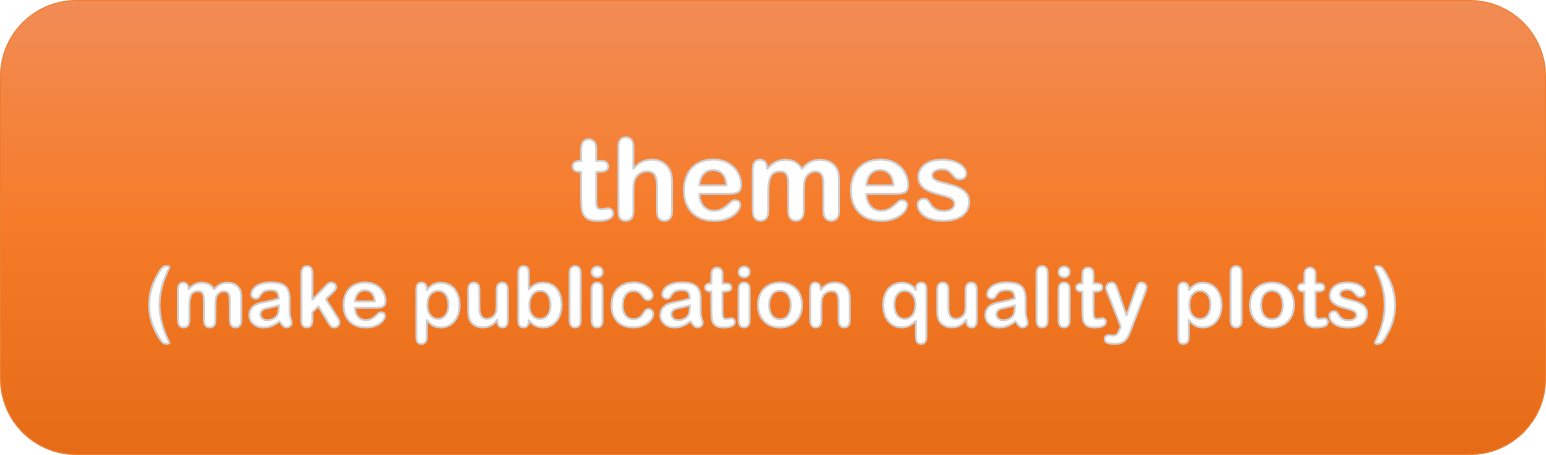
\includegraphics{/cloud/project/figures/themes.png}

\hypertarget{cleaning-up-plot}{%
\section{Cleaning up plot}\label{cleaning-up-plot}}

\hypertarget{add-axis-labels-and-title}{%
\subsection{add axis labels and title}\label{add-axis-labels-and-title}}

\includegraphics{Using_ggplot2_files/figure-latex/unnamed-chunk-52-1.pdf}

\hypertarget{default-themes}{%
\subsection{default themes}\label{default-themes}}

\includegraphics{Using_ggplot2_files/figure-latex/unnamed-chunk-53-1.pdf}

\includegraphics{Using_ggplot2_files/figure-latex/unnamed-chunk-54-1.pdf}

\hypertarget{save-plot}{%
\subsection{save plot}\label{save-plot}}

\hypertarget{bonus-animation}{%
\section{Bonus: Animation}\label{bonus-animation}}


\end{document}
